\section{Introduction}
Before talking about the main 3D-sensing techniques of autonomous navigation and metaverse, let’s talk about their history:

Autonomous Navigation \cite{autonomousHistory} — In the 1500 centuries before the invention of any modern technology, Leonardo da Vinci designed a cart, which is considered the world’s first robot that could move without being pushed or pulled. Years later in 1933, the demand for extended travel times forced the development of autopilot systems for long-range aircraft. Mechanical Mike was a prototype autopilot designed by Sperry Gyroscope Co. and used by Wiley Post during a 13,000-mile, around-the-world flight. In 1961, a Stanford engineering graduate student James Adams develop the world’s first truly self-driving wheeled vehicle, which was eventually outfitted with cameras and programmed to detect and autonomously follow a solid white line on the ground. And eventually, the most well-known Tesla autonomous driving car was introduced in late 2015.

\begin{figure}[H]
    \centering
    \subfigure{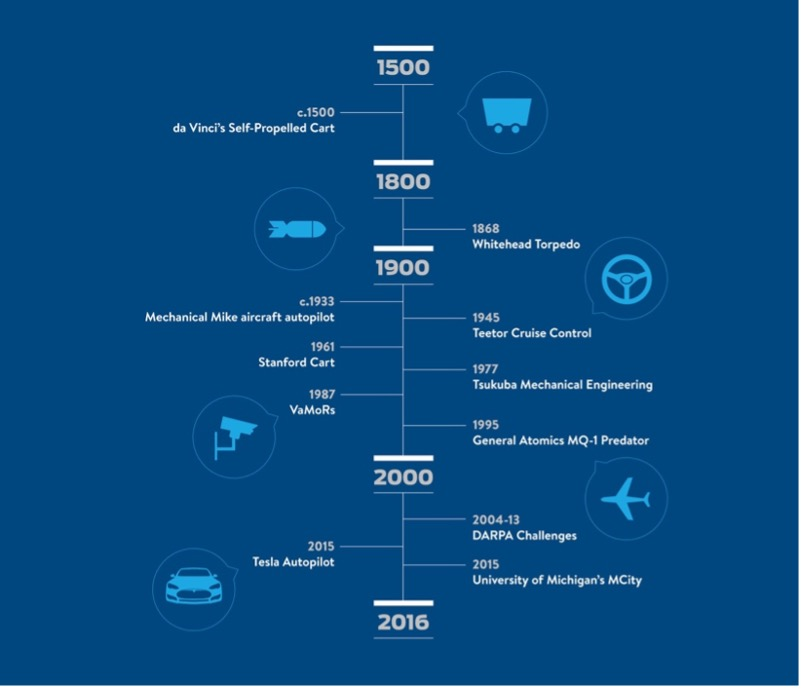
\includegraphics[width=.791\columnwidth]{autoHis}}
    \caption[Short text]{The history of Autonomous Navigation \cite{autonomousHistory}}
    \label{fig:autoHis}
\end{figure}

Metaverse \cite{metaverseHistory} — The term “metaverse” first comes from a sci-fi writer Neal Stephenson in 1992, to describe a 3D virtual space. While currently, the word “metaverse” is a digital world created by the infusion of different technologies like Virtual Reality (VR), Augmented Reality (AR), and the Internet. The most famous applications nowadays are Philip Rosedale's “Second Life” online virtual world in 2003 and Mark Zuckerberg's 2021 announcement of Meta's metaverse plan.

\begin{figure}[H]
    \centering
    \subfigure{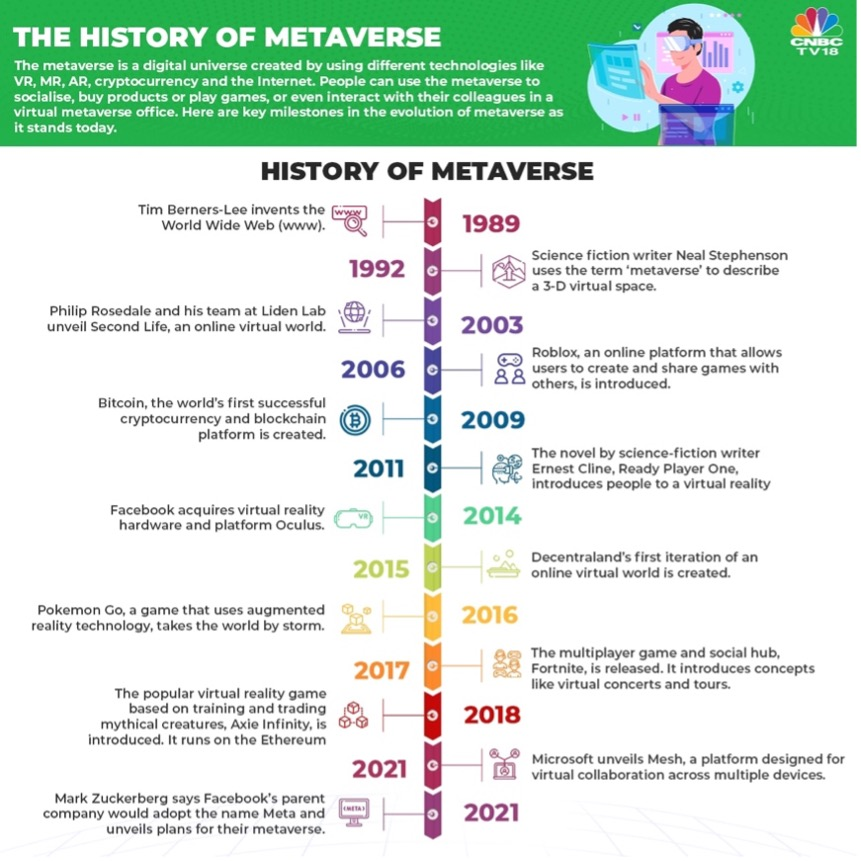
\includegraphics[width=.791\columnwidth]{metaverseHis}}
    \caption[Short text]{The history of Metaverse \cite{metaverseHistory}}
    \label{fig:metaverseHis}
\end{figure}